\documentclass[conference]{IEEEtran}
\IEEEoverridecommandlockouts

\usepackage{cite}
\usepackage{amsmath,amssymb,amsfonts}
\usepackage{graphicx}
\usepackage{textcomp}
\usepackage{xcolor}
\usepackage{url}


\begin{document}

\title{Towards Clinically Meaningful Explainability in ICU Time Series Prediction Models}

\author{
\IEEEauthorblockN{Shivani Muthukumaran}
\IEEEauthorblockA{
SEMTM0045 – Data Science Methods and Practice\\
University of Bristol}
}

\maketitle

\begin{abstract}
Time series models are widely used in Intensive Care Units (ICUs) to monitor patients and predict clinical deterioration from continuously recorded physiological data. Although deep learning models achieve high predictive performance, their lack of transparency limits their use in clinical settings where decisions must be interpretable and justifiable. Existing explainability methods, including SHAP and LIME, are commonly applied to these models; however, they treat temporal data as static and fail to capture dependencies across time, resulting in fragmented and clinically uninformative explanations.
This study evaluates the effectiveness of current explainability techniques for healthcare time series models in the context of ICU patient deterioration prediction. Specifically, it conducts a structured comparison of post-hoc methods (SHAP, LIME) and intrinsic approaches (attention-based and transformer models), assessing their ability to produce consistent, temporally coherent, and clinically meaningful explanations. The evaluation is designed around defined criteria, including faithfulness, stability under perturbations, and alignment with clinically relevant temporal patterns.
Building on these findings, the project proposes a conceptual framework that incorporates temporal importance into the explanation process by explicitly modelling feature contributions across time steps rather than treating them independently. By addressing the disconnect between predictive performance and interpretability, this research aims to support the development of more trustworthy decision-support systems in critical care, enabling clinicians to better understand, validate, and act upon model predictions in high-stakes environments.
\end{abstract}

\begin{IEEEkeywords}
Time Series Analysis, Explainable AI (XAI), Intensive Care Unit (ICU), Patient Deterioration Prediction, Model Interpretability, Temporal Dependencies, Healthcare Analytics
\end{IEEEkeywords}

\section{Introduction}
The growing use of continuous monitoring systems in ICUs has led to an increasing reliance on time series models to predict patient deterioration. Early identification of critical events such as sepsis or respiratory failure can significantly improve patient outcomes by enabling timely medical intervention. Deep learning models, particularly Long Short-Term Memory (LSTM) networks and Transformer-based architectures, have shown a strong capability to capture complex temporal patterns within multivariate clinical data. However, despite their predictive strength, their practical use in clinical settings remains limited.

One of the main challenges is lack of interpretability in high-risk environments like ICUs. Models that function as black boxes offer little transparency, making it difficult for healthcare professionals to trust or act upon their outputs. To address this, post-hoc explainability methods such as SHAP and LIME are often used to provide insights into model decisions.

Despite their widespread use, these methods are not well suited to time series data. They typically treat inputs as independent features and overlook the sequential nature of the data, resulting in explanations that fail to reflect how patient conditions evolve over time. In practice, this can lead to interpretations that are incomplete or difficult to apply in clinical decision-making, where the timing of changes is often as important as the changes themselves.

This highlights a gap between model performance and meaningful interpretability in healthcare applications. Although significant effort has been made to improve predictive accuracy, less attention has been paid to ensuring that explanations are temporally coherent and clinically useful. This project addresses this issue by evaluating existing explainability approaches for ICU time series models and proposing a framework to improve how temporal information is captured in model explanations. 

\footnote{\href{https://github.com/UoB-DSMP2026/research-portfolio-M-Shivani}}


\section{Literature Review}

\textbf{A.	Post-hoc Explainability Methods}\\
Post-hoc explainability methods such as SHAP and LIME are widely adopted due to their flexibility and model-agnostic nature. SHAP provides theoretically grounded feature attributions based on cooperative game theory, meanwhile LIME approximates local model behaviour using interpretable surrogate models \cite{lundberg2017shap,ribeiro2016lime}. These methods are frequently applied to complex models to provide insights into individual predictions.

However, both approaches are fundamentally designed for static tabular data and assume feature independence. When applied to time series models, they often treat sequential observations as independent inputs, ignoring temporal structure. This results in explanations that fail to reflect how patterns evolve over time. Such methods are not inherently suited for sequential data and may produce misleading interpretations in time-dependent contexts \cite{tschernutter2023timeseriesxai}. Furthermore, studies on explanation robustness demonstrate that widely used attribution methods can generate unstable or unreliable outputs under minor perturbations, raising concerns about their trustworthiness \cite{adebayo2018sanity}.\\

\textbf{B. Intrinsic Interpretability and Attention-based Models}\\
Researchers have studied intrinsic interpretability through attention-based systems and their interpretable model designs because post-hoc methods proved inefficient. Attention mechanisms enable systems to identify important moments and essential elements in a sequence, which provides users with straightforward results through their functioning. Attention-based models assess critical phases that patients experience during their medical journey, which they conduct through their clinical applications \cite{song2018attentive}. Temporal Fusion Transformers employ advanced architectures that use attention together with gating systems to achieve better system performance and improved system understanding \cite{lim2021temporal}.

The trustworthiness of attention systems as explanation mechanisms has not reached a conclusion despite the progress made so far. Attention weights cannot be used to determine which features matter most because they fail to deliver accurate descriptions of how models operate \cite{jain2019attention}. The literature contains a major conflict because researchers present attention systems as systems that provide interpretable results, yet these systems fail to deliver dependable explanations for their outcomes. The methods of intrinsic interpretability provide users with understandable information, but they lack the scientific evidence needed to establish themselves as trustworthy explanation methods.\\

\textbf{C. Healthcare Time Series Modeling}\\
Healthcare time series data analysis shows deep learning models which researchers use to study ICU data. The availability of large-scale datasets such as MIMIC-III has enabled the development of predictive models for patient deterioration \cite{johnson2016mimic}. Recurrent neural networks, especially LSTM-based models, have demonstrated strong performance in modeling sequential patient data \cite{lipton2015lstm}. The deep learning system successfully identifies complex time-based patterns which exist in electronic health records according to broader studies about its effectiveness \cite{shickel2017deep, fawaz2019dl4ts}.

The research studies which evaluate forecasting accuracy will show that most studies lack methods to explain their results. In clinical environments, this creates a significant barrier to adoption, as healthcare professionals require transparent and justifiable decision-support systems. Research on explainable AI in healthcare highlights that explanations must align with clinical reasoning and context, rather than simply providing numerical feature importance \cite{holzinger2017xaihealth}. The need for explanations arises from two requirements which demand technical validity and user-friendly understanding.\\

\textbf{D. Evaluation and Challenges in Explainability}\\
The literature shows a second limitation because researchers have not established standard procedures to assess explainability. Researchers argue that interpretability lacks proper scientific assessment methods which makes it impossible to determine whether explanations meet validity and usefulness standards according to \cite{doshi2017rigorous}. The evaluation process requires assessment of both feature importance and temporal evaluation in time series analysis.

The scientific community continues to debate whether researchers should present explanations for black-box systems or develop models that offer direct interpretability. Some research indicates that post-hoc explanations create misleading understanding which particularly affects high-stakes fields like healthcare according to \cite{rudin2019stop}. The perspective shows a need for explanation methods which demonstrate accurate model performance while meeting actual decision-making needs.

\section{Research Gap and Objectives }

\textbf{A.	Research Gap}\\
The literature reveals a clear disconnect between predictive performance and meaningful interpretability in healthcare time series models. While post-hoc methods provide flexible explanations, they fail to capture temporal dependencies and often produce fragmented interpretations. Intrinsic approaches attempt to address this limitation but lack consistency and reliability as explanation mechanisms. At the same time, healthcare-focused studies prioritize accuracy over interpretability, resulting in models that are difficult to trust and apply in clinical settings. These observations are also seen in papers \cite{arrieta2020xai,wachter2017counterfactual,guidotti2018survey,hewamalage2021forecasting,tonekaboni2019clinicians,topol2019aihealthcare}.

Moreover, there is no widely accepted framework for evaluating the quality of explanations, particularly in sequential data contexts. Existing approaches rarely consider whether explanations are coherent or clinically meaningful. As a result, current methods are insufficient to support real-world decision-making in ICU environments.\\

\textbf{B.	Research Question}\\
How can explainability methods be adapted or enhanced to capture temporal dependencies and provide clinically meaningful interpretations for ICU time series prediction models?\\

\textbf{C.	Objectives}

1. Critically evaluate the existing explanation methods applied to time series models in healthcare.

2. Analyze the limitations of these methods in capturing temporal dependencies and producing consistent and clinically meaningful explanations.

3.	Propose a conceptual framework for temporally-aware explainability, incorporating feature importance across time steps.

4.	Define evaluation criteria for assessing explanation quality, including faithfulness, stability and clinical interpretability.



\section{Proposed Methodology}
This study adopts a benchmark-and-enhance approach, where standard time series models and explainability methods are used as baselines, followed by the development of a temporally aware explanation framework to improve interpretability in ICU prediction tasks.\\

\begin{figure}
    \centering
    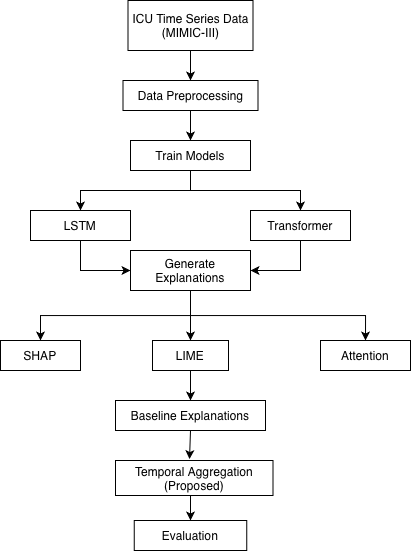
\includegraphics[width=1\linewidth]{Proposed Pipeline.drawio.png}
    \caption{Proposed Pipeline}
    \label{fig:placeholder}
\end{figure}

\textbf{A. Technical Pipeline}
The proposed methodology consists of four main stages:

1. Data Preparation: 
Multivariate ICU time series data (e.g., vital signs, laboratory measurements) will be extracted and preprocessed using
\begin{itemize}
    \item Missing value imputation
    \item Normalisation
    \item Segmentation into fixed-length temporal windows
\end{itemize}

2. Predictive Modeling:
Two baseline models will be implemented for the next stage
\begin{itemize}
\item LSTM model for sequential learning \cite{lipton2015lstm}
\item Temporal Fusion Transformer (TFT) for capturing complex temporal dependencies \cite{lim2021temporal}
\end{itemize}

These models provide a strong benchmark for ICU deterioration prediction.

3. Baseline Explainability:
Model predictions will be interpreted using
\begin{itemize}
    \item SHAP and LIME (post-hoc explanations) \cite{lundberg2017shap, ribeiro2016lime}
    \item Attention weights from transformer models
\end{itemize}

4. Proposed Enhancement:

To address the lack of temporal awareness in explanations, the following improvements are introduced

a) Temporal Aggregation of Explanations: Feature importance scores will be aggregated across time steps to capture:
\begin{itemize}
    \item temporal trends
    \item persistence of feature influence
\end{itemize}
This shifts explanations from isolated feature attribution to time-dependent importance profiles.

b) Time-window-based Interpretation: Instead of analysing individual timestamps, explanations will be grouped into clinically meaningful time windows (e.g., early vs late deterioration phases), improving interpretability.

c) Temporal Coherence Analysis: A new evaluation dimension is introduced to measure whether the explanation patterns evolve smoothly and meaningfully over time.\\

\textbf{B. Justification of Approach}

The selection of LSTM and Transformer models is based on their established effectiveness in modeling healthcare time series data \cite{lipton2015lstm, lim2021temporal}. Using these as baselines ensures that the study is grounded in current best practices. Similarly, SHAP and LIME are chosen due to their widespread adoption in explainability research. Rather than replacing these methods, the proposed approach extends them, making the solution compatible with existing workflows and easier to adopt in real-world systems.
The introduction of temporal aggregation and coherence analysis directly addresses the need for time-aware interpretability, which is not explicitly handled by standard methods.\\

\textbf{C. Evaluation Strategy}

The proposed framework will be evaluated through a comparative analysis against baseline explainability methods. The objective is to assess whether incorporating temporal information improves the quality and usability of model explanations.

\begin{itemize}
    \item Faithfulness: Whether explanations accurately reflect model behaviour, tested through feature perturbation.
    \item Robustness: Stability of explanations under minor input variations.
    \item Proposed Temporal Consistency: Ability to capture coherent patterns across time rather than isolated feature importance.
    \item Clinical Relevance: Alignment of explanations with expected medical reasoning.
\end{itemize}
Expected outcome: This approach is expected to produce more consistent and interpretable explanations by capturing temporal patterns, thereby improving their usefulness in clinical decision-making.



\section{Data, Ethics, and Practical Considerations}

\textbf{A. Data Readiness}\\

The study will use the MIMIC-III dataset which serves as a common public ICU database that contains anonymized patient data according to  \cite{johnson2016mimic}. The dataset contains high-resolution multivariate time series data which includes vital signs and laboratory measurements and clinical interventions. It allows researchers to create patient deterioration models through its complete set of vital signs, laboratory results and medical procedures. 
\begin{itemize}
    \item Availability: The system grants access to authenticated users to use its resources. 
    \item Data Quality: The clinical data shows actual patient information which contains both noise elements and missing data points as well as irregular intervals of data collection. 
    \item Suitability: The dataset contains extensive time-based information which meets the requirements needed for time series analysis. 
    \item Licensing: It received approval for its data usage under particular research terms and conditions. 
Despite its strengths, pre-processing is required to handle missing data, temporal misalignment, and class imbalance.
\end{itemize}

\vspace{0.3cm}

\textbf{B.  Ethical Red-Teaming}\\

An anticipatory evaluation of risks linked to the suggested system identifies several concerns:
\begin{itemize}
    \item Data Bias: Unequal representation among demographic groups might result in skewed predictions.
    \item Misleading Explanations: Unreliable or inaccurate explanations could foster misplaced confidence in model results.
    \item Privacy Risks: Even though data is de-identified, the possibility of re-identification still exists.
    \item Excessive dependence on AI: Medical professionals might place too much trust on model predictions during critical decision-making in high-stakes decisions.
\end{itemize}

\vspace{0.3cm}

\textbf{C. Technical and Procedural Mitigations}\\

To address these risks, the following safeguards are proposed:

\begin{itemize}
    \item Bias Mitigation: Evaluate model performance across demographic subgroups and report disparities
    \item Explanation Validation: Use robustness and faithfulness checks to ensure reliability of explanations
    \item Data Security: Adhere to data governance protocols and secure storage standards
    \item Human Oversight: Position the system as a decision-support tool, not a replacement for clinical judgment
\end{itemize}

\section{Project plan}

The project plan follows a structured 12-week lifecycle, progressing from literature review and data preparation to model development, explainability analysis, and final evaluation. Early stages focus on understanding the dataset and establishing baseline models, which form the foundation for subsequent explainability experiments. The proposed temporal aggregation framework is developed only after baseline methods are evaluated, ensuring that improvements are grounded in identified limitations. Tasks are organised with clear dependencies, where each phase builds upon the outputs of the previous stage, reducing redundancy and ensuring efficient use of time. The use of existing datasets, established models, and widely available tools further supports feasibility. Overall, the plan demonstrates that the project can be realistically completed within the given time frame while allowing sufficient scope for evaluation and refinement.\\

\begin{figure}
    \centering
    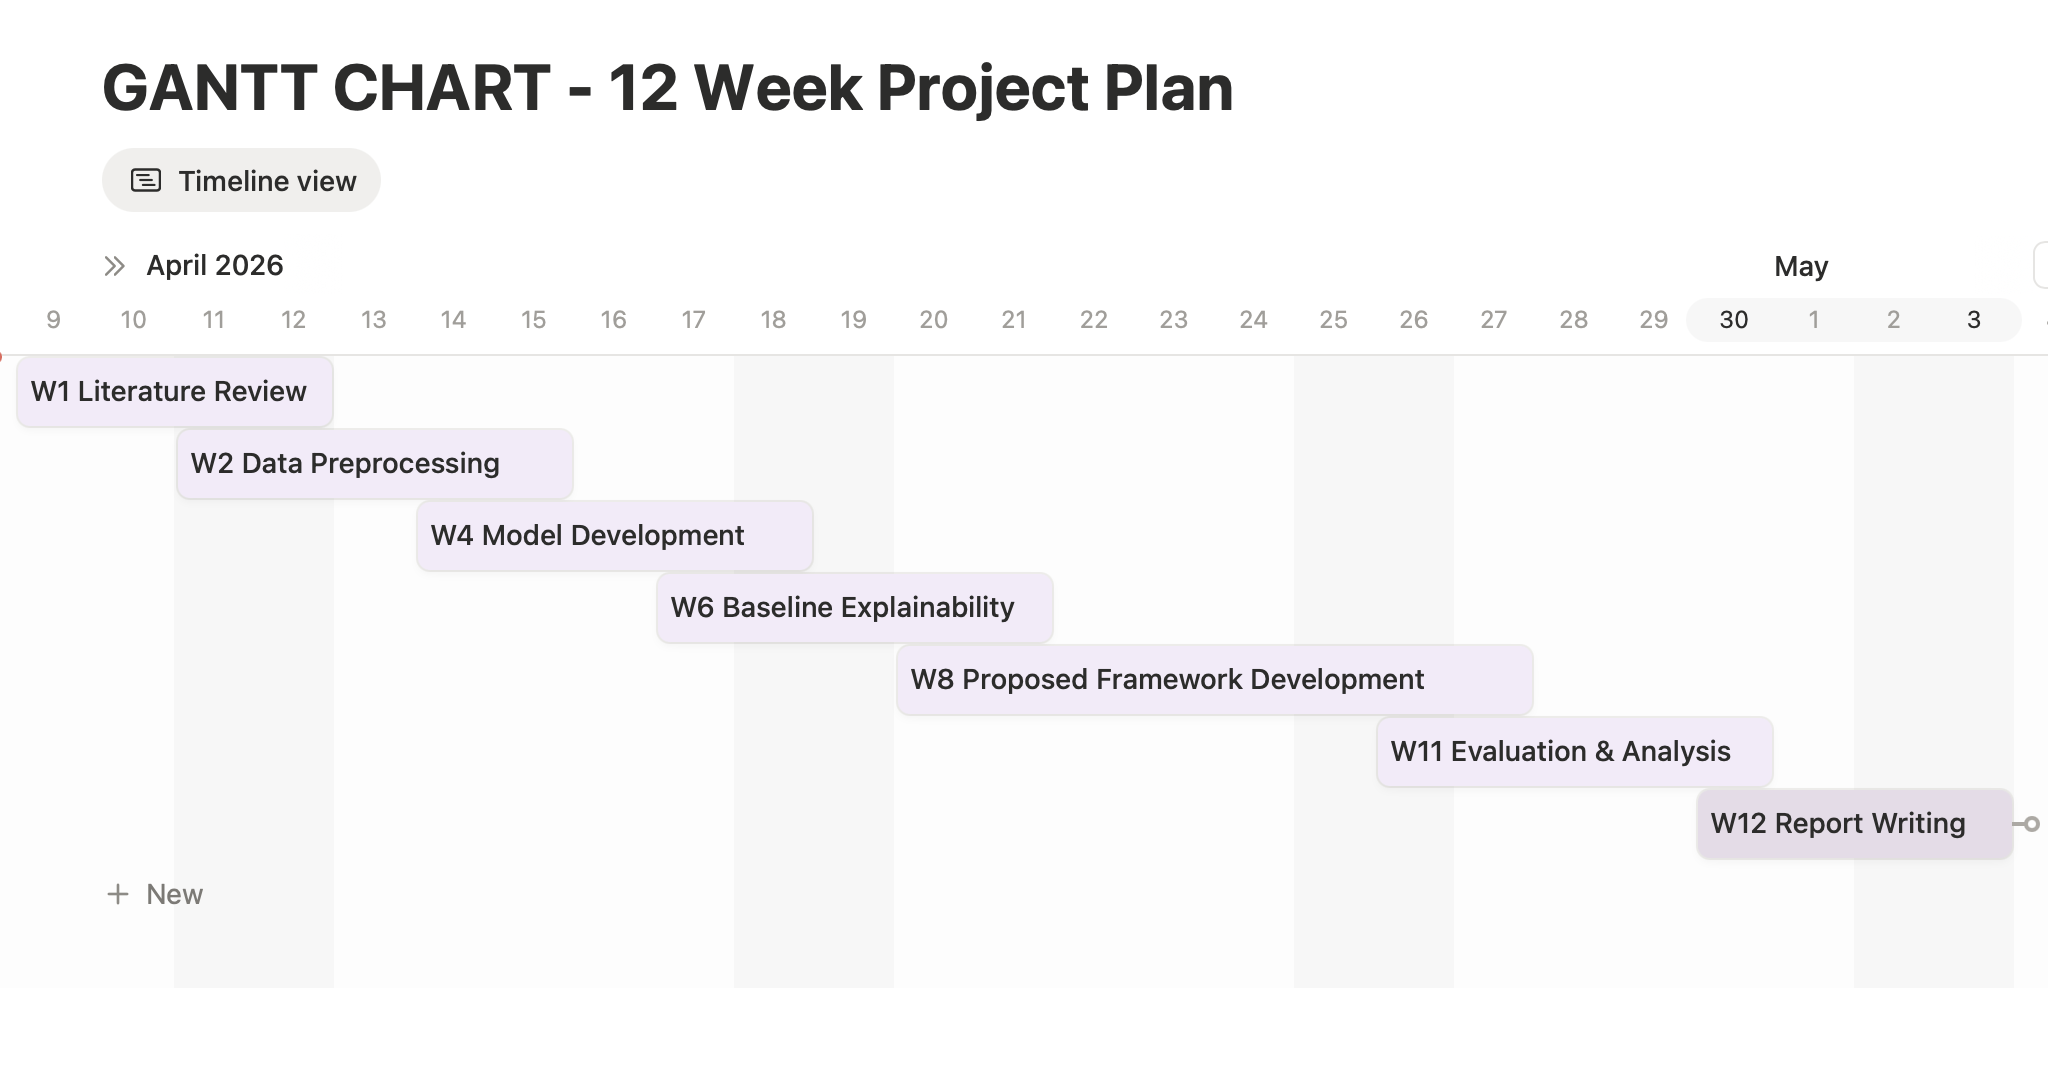
\includegraphics[width=1.15\linewidth]{Gantt Chart.png}
    \caption{Gantt Chart for Project Timeline}
    \label{fig:placeholder}
\end{figure}


The project plan is managed using Notion and can be accessed at:
\href{https://www.notion.so/Research-Project-Plan-33c75170ef8f801ebf35fde19827464a}

\section{Non-Technical Summary}

In modern hospitals, particularly in Intensive Care Units (ICUs), large amounts of patient data are continuously collected, including vital signs such as heart rate, blood pressure, and oxygen levels. Advanced computer models are increasingly used to analyse this data and predict when a patient’s condition might worsen. While these models can be highly accurate, they often function as “black boxes,” meaning that clinicians cannot easily understand how or why a particular prediction was made. This lack of transparency limits trust and makes it difficult to rely on these systems in critical, life-or-death situations.

This project focuses on improving how these predictions are explained to healthcare professionals. Instead of only providing a prediction, the goal is to show why the model reached that conclusion, in a way that reflects how a patient’s condition changes over time. Current explanation methods tend to treat patient data as static snapshots, which can result in confusing or incomplete insights. This research aims to address this issue by developing a method that highlights how important factors evolve over time, making explanations more meaningful and easier to interpret.

The expected outcome is a more transparent and reliable decision-support tool that helps clinicians better understand model predictions. This can support earlier detection of patient deterioration, more informed decision-making, and ultimately improved patient outcomes. By making artificial intelligence systems more interpretable and trustworthy, this work contributes to safer and more effective use of technology in healthcare, where clarity and accountability are essential.

\bibliographystyle{IEEEtran}
\bibliography{references}


\end{document}
